\begin{frame}
  \frametitle{Sparse Grids -- Basics}
  \topline
  \vspace{-10px}
  \begin{block}{Hirachial Basis}
    \begin{figure}[!htp]
      \setbeamertemplate{caption}{\raggedright\insertcaption\par}
      \setbeamerfont{caption}{size=\footnotesize}
      \centering
      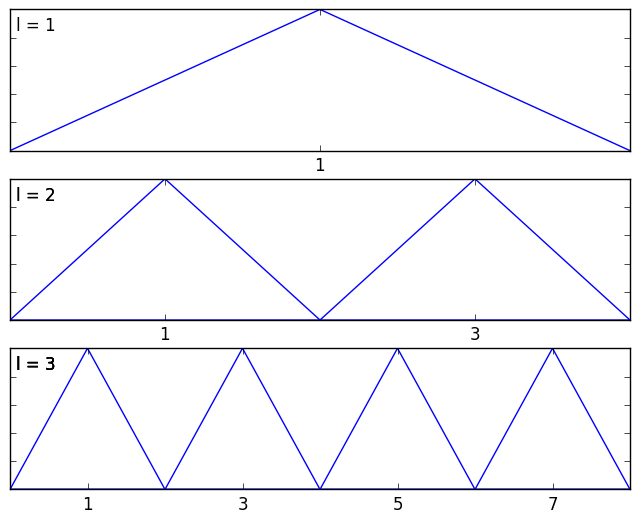
\includegraphics[width=7.5cm]{images/sparse_hats}
      \vspace{-12px}
      \caption{}
    \end{figure}
  \end{block}
\end{frame}

\begin{frame}
  \frametitle{Sparse Grids -- Basics}
  \topline
  \vspace{-10px}
  \begin{block}{Hirachial basis (vs nodal basis)}
    \begin{itemize}
      \item Grouping gridpoints into levels $l \in \{1,2,3\dots\}$
      \item Basis function by index \textbf{and} level: $\phi_{l,i}(x)$
    \end{itemize}
    \vspace{20px}
    \begin{center}
      $\hat{f}(x) = \sum_{l,i}{\ \alpha_{l,i} \cdot \phi_{l,i}(x)}$
    \end{center}
  \end{block}
\end{frame}

\begin{frame}
  \frametitle{Sparse Grids -- Basics}
  \topline
  \vspace{-10px}
  \begin{block}{Hirachial Basis}
    \begin{figure}[!htp]
      \setbeamertemplate{caption}{\raggedright\insertcaption\par}
      \setbeamerfont{caption}{size=\footnotesize}
      \centering
      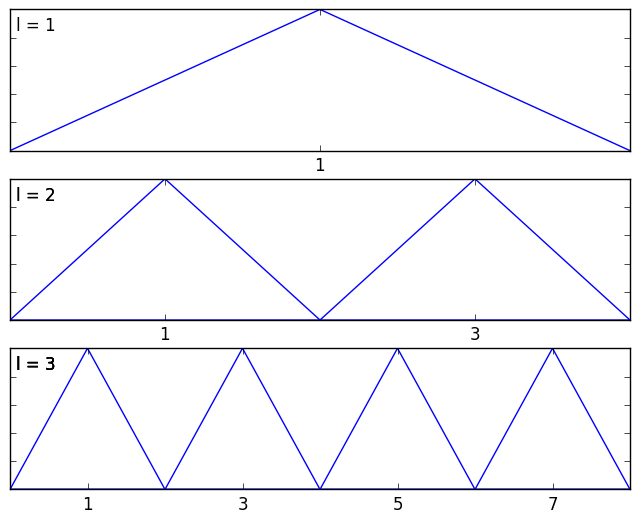
\includegraphics[width=7.5cm]{images/sparse_hats}
      \vspace{-12px}
      \caption{}
    \end{figure}
  \end{block}
\end{frame}

\begin{frame}
  \frametitle{Sparse Grids -- Basics}
  \topline
  \vspace{-10px}
  \begin{block}{Hirachial vs. nodal  basis}
    \begin{figure}[!htp]
      \setbeamertemplate{caption}{\raggedright\insertcaption\par}
      \setbeamerfont{caption}{size=\footnotesize}
      \centering
      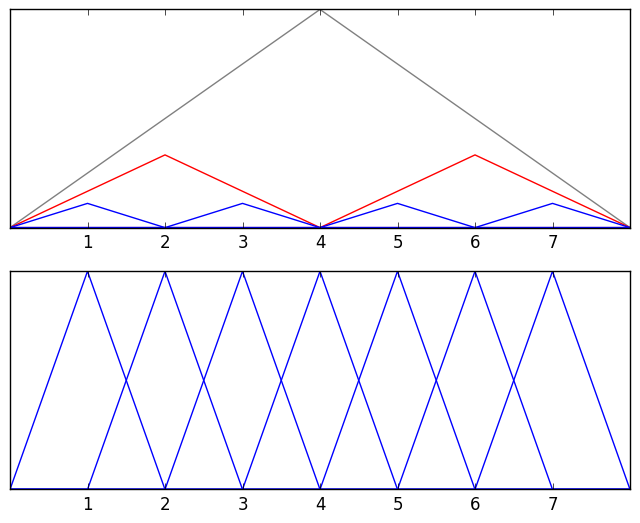
\includegraphics[width=7.5cm]{images/sparse_together}
      \vspace{-12px}
      \caption{}
    \end{figure}
  \end{block}
\end{frame}

\begin{frame}
  \frametitle{Sparse Grids -- Basics}
  \topline
  \vspace{-10px}
  \begin{block}{Basis function subspaces}
    \begin{itemize}
      \item Combination of levels through all dimensions
    \end{itemize}
  \end{block}
\end{frame}

\begin{frame}
  \frametitle{Sparse Grids -- Basics}
  \topline
  \vspace{-10px}
  \begin{block}{Hirachical gridpoints}
    \begin{figure}[!htp]
      \setbeamertemplate{caption}{\raggedright\insertcaption\par}
      \setbeamerfont{caption}{size=\footnotesize}
      \centering
      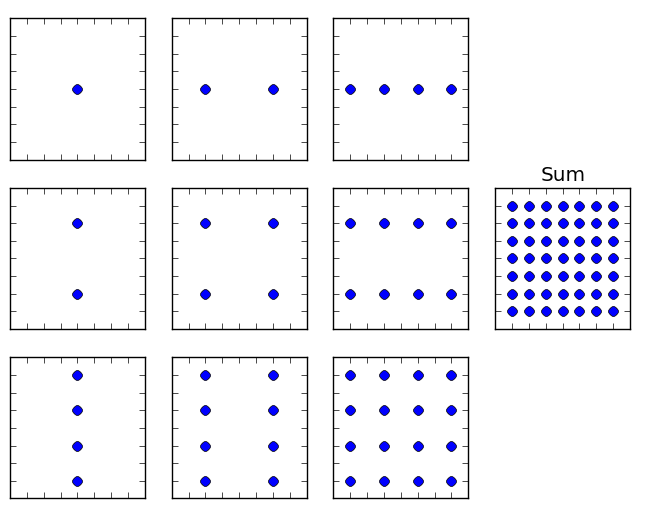
\includegraphics[width=7.5cm]{images/sparsegrid_hirach1}
      \vspace{-12px}
      \caption{}
    \end{figure}
  \end{block}
\end{frame}

\begin{frame}
  \frametitle{Sparse Grids -- Basics}
  \topline
  \vspace{-10px}
  \begin{block}{Hirachical subspaces}
    \begin{figure}[!htp]
      \setbeamertemplate{caption}{\raggedright\insertcaption\par}
      \setbeamerfont{caption}{size=\footnotesize}
      \centering
      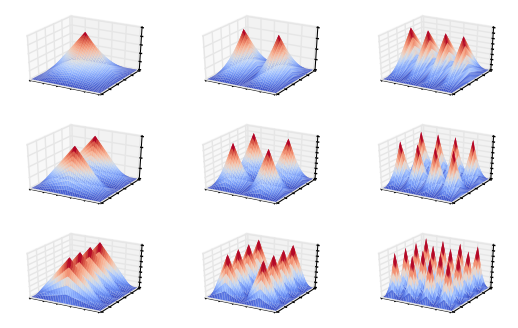
\includegraphics[width=7.5cm]{images/sparsegrid_2dhats}
      \vspace{-12px}
      \caption{}
    \end{figure}
  \end{block}
\end{frame}

\begin{frame}
  \frametitle{Sparse Grids -- Basics}
  \topline
  \vspace{-10px}
  \begin{block}{Sparse grid -- Changes}
    \begin{itemize}
      \item Throwing away certain subspaces
      \item Finding those is a \emph{a-priori} solvable optimization problem
      \item The resulting gird is now \textbf{sparse}
      \end{itemize}
  \end{block}
  \begin{block}{Profit}
    \begin{itemize}
      \item Reducing the computational effort ``a lot''
      \item Maintaining ``high'' accuracy
      \end{itemize}
  \end{block}
\end{frame}

\begin{frame}
  \frametitle{Sparse Grids -- Basics}
  \topline
  \vspace{-10px}
  \begin{block}{A \emph{sparse} grid}
    \begin{figure}[!htp]
      \setbeamertemplate{caption}{\raggedright\insertcaption\par}
      \setbeamerfont{caption}{size=\footnotesize}
      \centering
      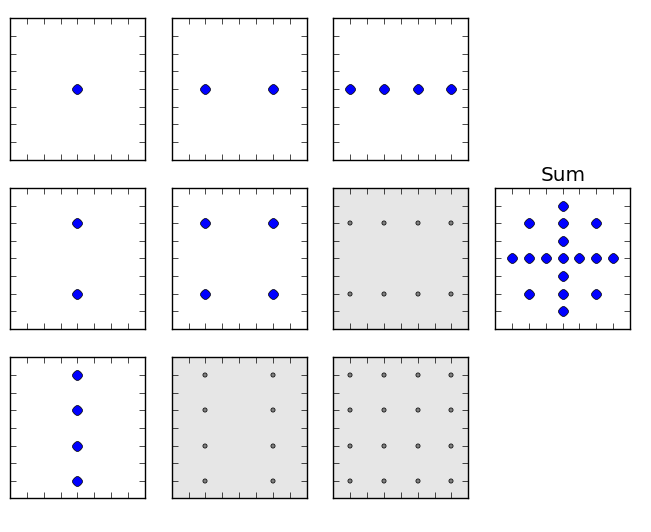
\includegraphics[width=7.5cm]{images/sparsegrid_hirach2}
      \vspace{-12px}
      \caption{}
    \end{figure}
  \end{block}
\end{frame}

\begin{frame}
  \frametitle{Sparse Grids -- Basics}
  \topline
  \vspace{-10px}
  \begin{block}{Boundry and smoothness}
    \begin{itemize}
      \item Boundries need special treatment
      \item The function needs to be sufficient smooth \\
        $D^2f$ need to be bounded
      \end{itemize}
  \end{block}
  \begin{block}{Adaptivity}
    \begin{itemize}
      \item \emph{A-posteriori} modifications to better fit the function
      \item Picking a single gridpoint and adding level of detail around it
      \item Prone to overfitting and huge computational effort
      \end{itemize}
  \end{block}
\end{frame}


\begin{frame}
  \frametitle{Sparse Grids -- Basics}
  \topline
  \vspace{-10px}
  \begin{block}{Summary}
    \begin{itemize}
      \item Hirachial basis through grouping gridpoints into levels
      \item Creating ``subspaces'' through combination of levels in dimensions
      \item Selecting and combining subspaces
      \end{itemize}
  \end{block}
  \begin{block}{To keep in mind}
    \begin{itemize}
      \item Smoothness requirement for $f(x)$
      \item Boundry treatment
      \item Accuracy--effort trade-off
      \item Adaptivity options (\emph{a-posteriori})
      \end{itemize}
  \end{block}
\end{frame}



%%% Local Variables:
%%% TeX-master: "slides"
%%% End:
